\chapter{Complete Programming Stack Verification}
\graphicspath{ {./images/}} 

A computing programming stack being referred here is basically classical toolchain that includes all the tools from low level to high level. It includes compilers, linkers, debuggers, Database Management System (DBMSS) and interfacing kernels. The idea of stack verification is to check the correctness of all these technologies. Assuming the logical model of each of the software we can use the reasoning of Curry-Howard correspondence and Hoare Logic to construct a verifiable proof for each one.\\

\section{DeepSpec Project}


\begin{figure}[!htb]
\centering
  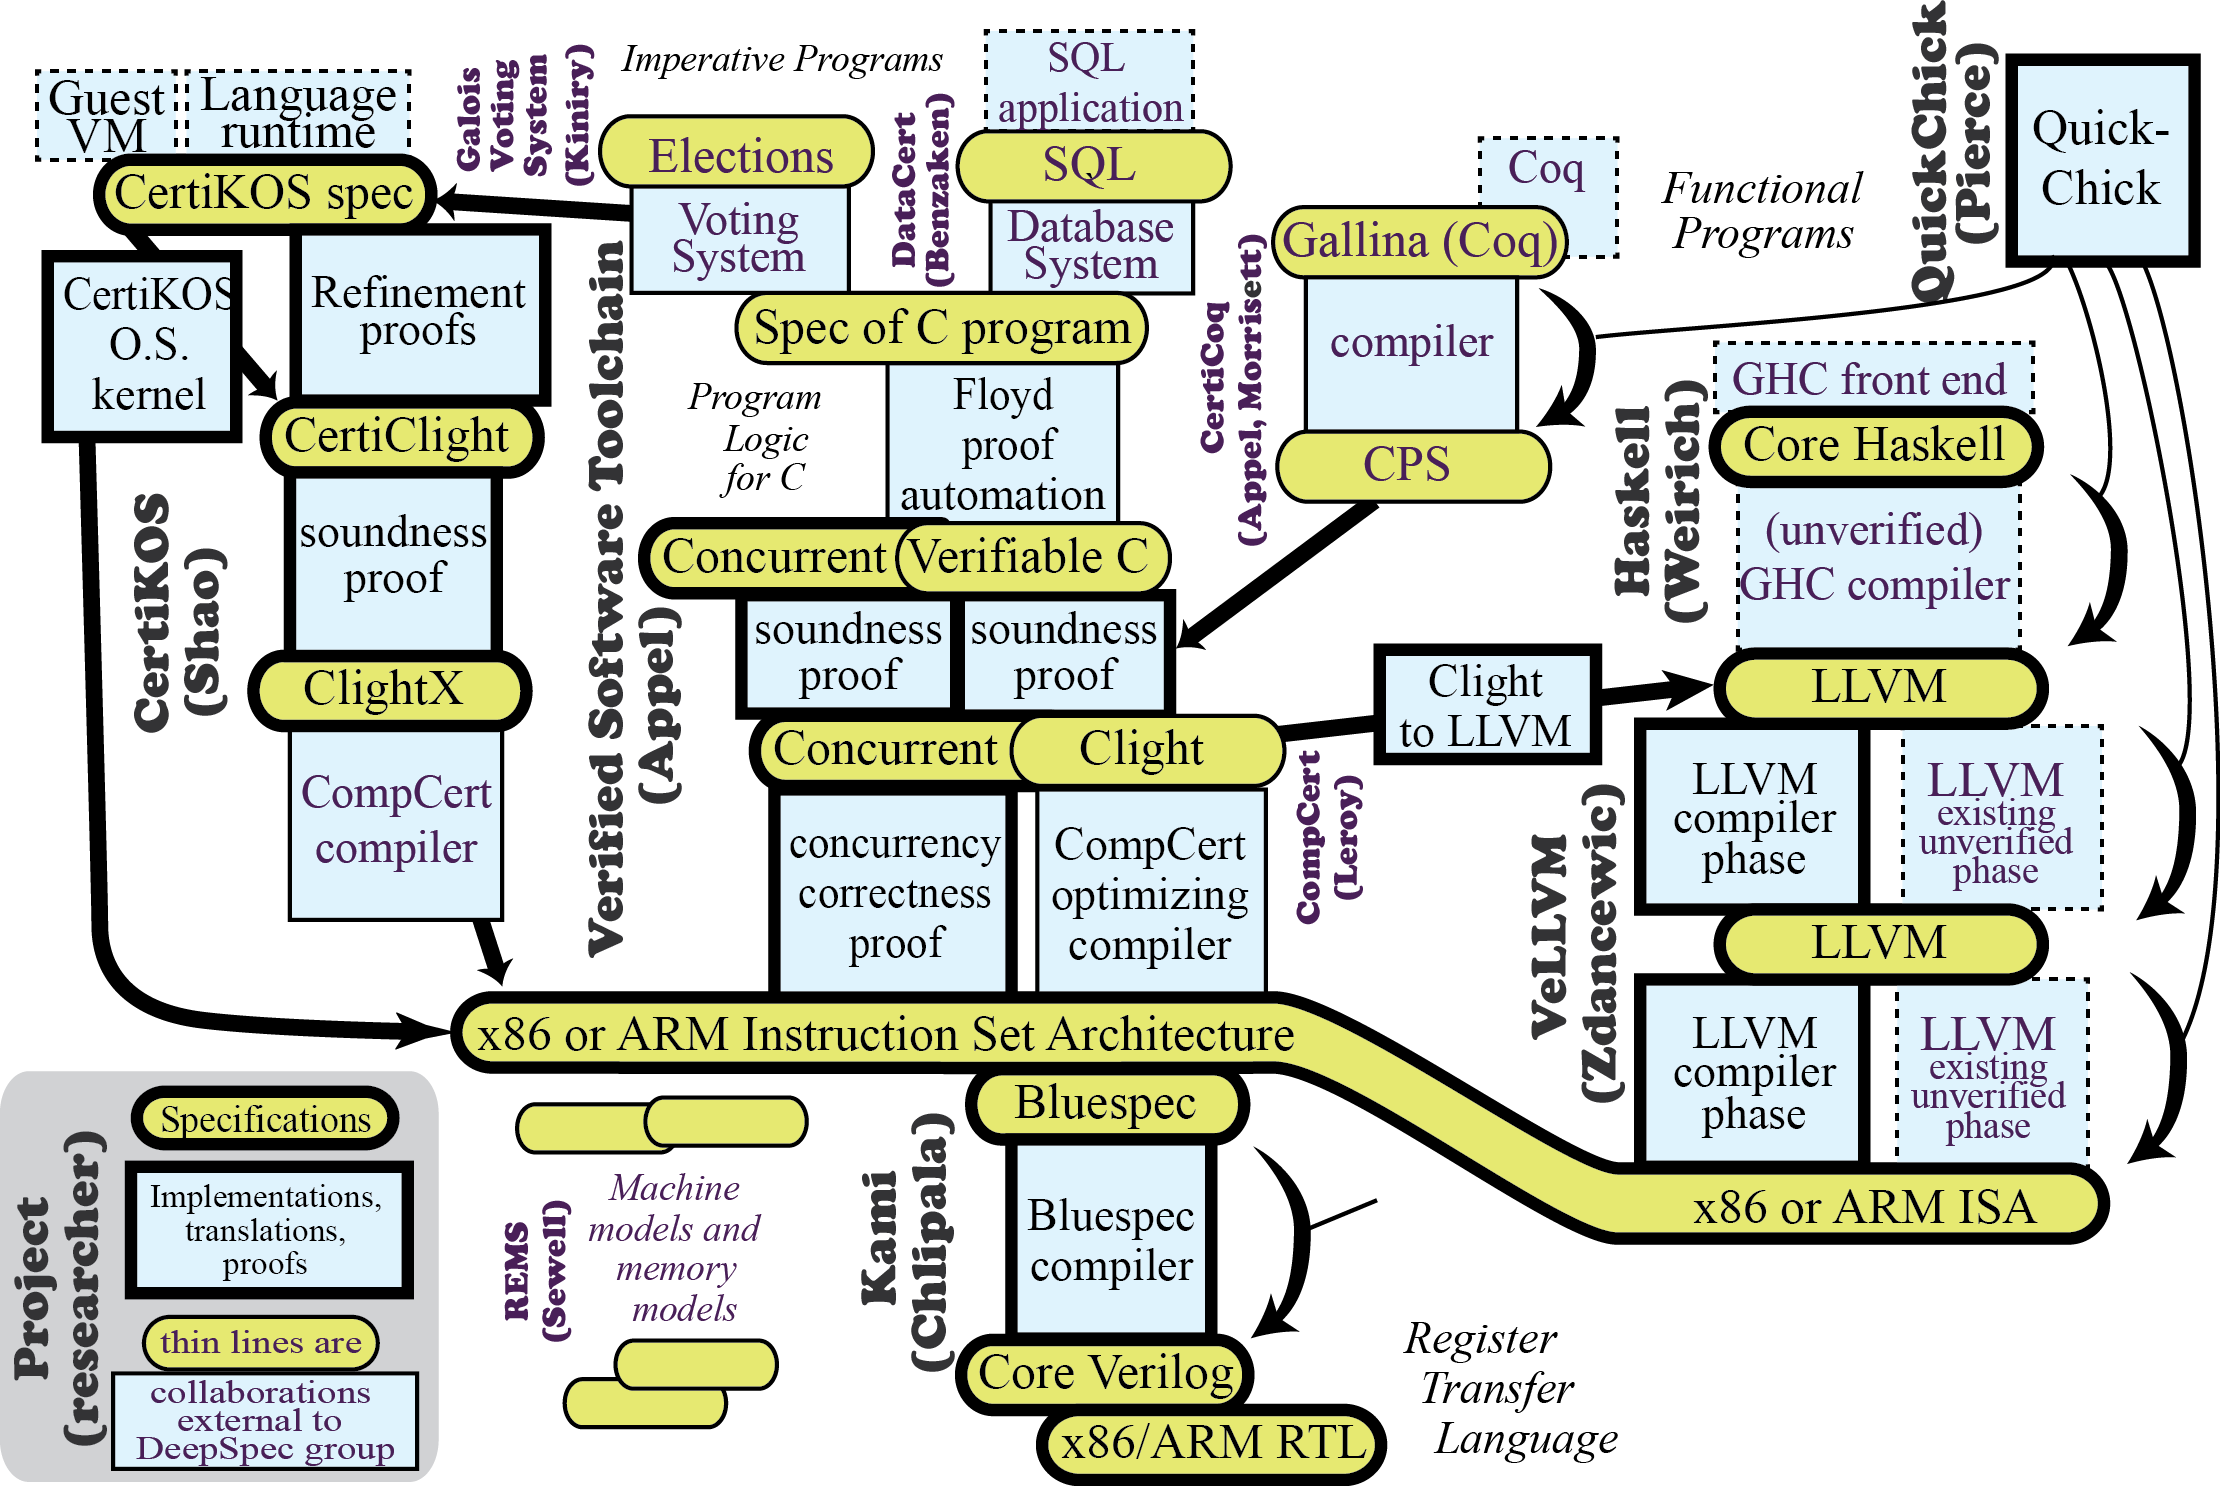
\includegraphics[scale=0.7]{deepspec}
  \caption{The DeepSpec Project}
\end{figure}

This project is umbrella project of many important projects like CertiCoq, VST, VELLVM, CertiKOS in the field of software verification. The subprojects deal with checking different software tools and also the operating system semantics. Thus the project DeepSpec overall verifies the computer stack. \\

A very basic explaination reads as provided in the manual, :

At the top of the diagram are specifications of application-level interfaces such as the semantics of the SQL query language or the rules governing fair Elections. At the bottom is the semantics of the RTL (register-transfer language) implementation of some specific microprocessor, say x86. A voting or database system is implemented as a C program with a specification Spec of C program, written in a program logic called Verifiable C. We prove (in Coq) that the C program correctly implements SQL by applying the program logic to the program, with the assistance of the Floyd proof automation system. Verifiable-C is a set of reasoning rules for program correctness; whatever properties are proved about a program will actually hold when the program runs; this is formalized in Coq as the soundness proof connecting Verifiable C to the operational semantics of C-light. The CompCert optimizing compiler compiles C light to machine language in ARM, PowerPC, or x86-ISA. The correctness of CompCert's translation is proved in Coq. Finally, the hardware is correct: the instruction set architecture x86-ISA is specified in the Bluespec hardware-description language, which itself has a deep specification defining its precise semantics. The Kami synthesizer translates this to register transfers written in Verilog (which, again, itself has a deep specification).\\

It would be a major breakthrough to completely build a coherent system of specified/verified components whose specification deals only with the semanics of some very basic technologies like for example Verilog and SQL.\\


